\documentclass[border=2pt]{standalone}
\usepackage{pgfplots}
\pgfplotsset{compat=1.18}
\begin{document}
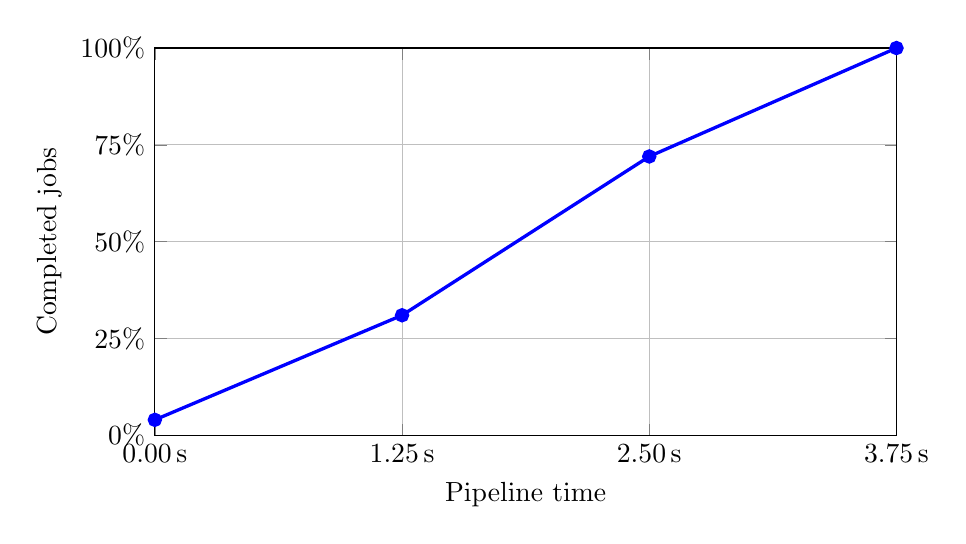
\begin{tikzpicture}
  \begin{axis}[
    width=11cm,
    height=6.5cm,
    xmin=0,
    xmax=3.75,
    ymin=0,
    ymax=100,
    xtick={0,1.25,2.5,3.75},
    xticklabel={$\pgfmathprintnumber[fixed,fixed zerofill,precision=2]{\tick}\,\mathrm{s}$},
    ytick={0,25,50,75,100},
    yticklabel={$\pgfmathprintnumber[fixed,precision=1]{\tick}\%$},
    grid=major,
    xlabel={Pipeline time},
    ylabel={Completed jobs}
  ]
    \addplot[blue,very thick,mark=*] coordinates {
      (0,4) (1.25,31) (2.5,72) (3.75,100)
    };
  \end{axis}
\end{tikzpicture}
\end{document}
